\documentclass[11pt,a4paper]{article}
\usepackage[utf8]{inputenc}
\usepackage[margin=1in]{geometry}
\usepackage{amsmath,amssymb,amsfonts}
\usepackage{booktabs}
\usepackage{graphicx}
\usepackage{hyperref}
\usepackage{microtype}
\usepackage{siunitx}
\usepackage{cite}
\usepackage{tikz}
\usepackage{xcolor}
\usepackage{enumitem}
\usepackage{fancyhdr}
\usepackage{tcolorbox}
\usepackage{array}

\pagestyle{fancy}
\fancyhf{}
\setlength{\headheight}{15pt}
\lhead{\textbf{NCSSM Connect Program} $\cdot$ Honors Aerospace Engineering}
\rhead{\textbf{WindTunnel lab} $\cdot$ Stall Lab Consortium}
\cfoot{\thepage}

\hypersetup{
    colorlinks=true,
    linkcolor=blue!70!black,
    citecolor=blue!70!black,
    urlcolor=blue!70!black
}

\tcbset{
    colback=gray!6!white,
    colframe=blue!70!black,
    fonttitle=\bfseries,
    boxrule=1pt,
    arc=4pt,
    left=8pt, right=8pt, top=8pt, bottom=8pt
}

\title{\vspace{-1.0cm}\textbf{\huge Collaborative Wind Tunnel Flight Investigation} \\[0.3cm]
\Large Multi-Variable Functional Scaling of Aerodynamic Stall \\[0.2cm]
\large $\alpha_{\text{stall}} = f(\alpha,\, m,\, t/c,\, Re)$ \\
\vspace{0.3cm}
\normalsize \textbf{Platform:} NCSSM \textit{WindTunnel lab} (GPU-Accelerated 2D Lattice Boltzmann Simulator)}
\author{\textbf{Developed by F. Santibanez, Ph.D.} \\
Honors Aerospace Engineering $\cdot$ NCSSM Connect Program \\
North Carolina School of Science and Mathematics}
\date{Academic Year 2026--2027}

\begin{document}
\maketitle

\begin{tcolorbox}[title=Mission Briefing \& Research Objective, colframe=blue!60!black]
In computational aerodynamics and experimental flight testing, \textbf{aerodynamic stall} represents the catastrophic loss of lift and surge in pressure drag resulting from massive boundary layer separation. While idealized thin-airfoil theory predicts an unyielding linear lift curve $C_L(\alpha) = 2\pi(\alpha - \alpha_0)$, physical fluids cannot overcome the adverse pressure gradient on the suction surface indefinitely.

As an aerospace research team, our class is commissioned to map the \textbf{functional response surface} of the critical stall angle:
\begin{equation}
\alpha_{\text{stall}} = \Phi\left(m,\, \frac{t}{c},\, Re\right), \quad \text{and the maximum achievable lift} \quad C_{L,\max} = \Psi\left(m,\, \frac{t}{c},\, Re\right)
\end{equation}
where $m$ is maximum airfoil camber, $t/c$ is the maximum thickness ratio, and $Re$ is the chord Reynolds number. To accomplish this broad parametric exploration, the class will operate as an \textbf{Aerodynamics Research Consortium} divided into four specialized test divisions. Each division will interrogate one parametric axis, share verified digital flight telemetry, and collaborate on a unified global regression model.
\end{tcolorbox}

\section{Aerodynamic Theory \& Physical Foundations}

\subsection{Lifting Airfoil Kinematics and Classical Limits}
According to classical Kutta-Joukowski lift theory and 2D thin-airfoil theory, for an inviscid, attached flow around a slender foil with mean camber line $y_c(x)$, the sectional lift coefficient is linear:
\begin{equation}
C_L(\alpha) = 2\pi (\alpha - \alpha_0) = a_0 (\alpha - \alpha_0), \quad a_0 \approx 2\pi \approx 6.28\,\text{rad}^{-1} \approx 0.110\,\text{deg}^{-1},
\end{equation}
where $\alpha_0$ represents the zero-lift angle of attack. For NACA 4-digit airfoils parameterized by maximum camber $m$ (expressed as a fraction of chord) located at chordwise station $p$, thin airfoil theory yields the integral:
\begin{equation}
\alpha_0 = -\frac{1}{\pi} \int_0^\pi \frac{dy_c}{dx} (\cos\theta - 1)\, d\theta \approx -k_c \cdot m, \quad (k_c \approx 1.05 \text{ to } 1.15 \text{ rad/unit camber}).
\end{equation}
Hence, camber translates the lift curve to the left, generating positive lift at $\alpha = 0^\circ$.

\subsection{Adverse Pressure Gradients and Boundary Layer Separation}
In a real viscous fluid, fluid deceleration downstream of the suction peak generates an adverse pressure gradient:
\begin{equation}
\frac{dp}{dx} > 0 \implies \mu \frac{\partial^2 u}{\partial y^2} > 0 \quad \text{at the wall } (y=0).
\end{equation}
Because viscous dissipation continuously strips kinetic energy from the near-wall fluid, the wall shear stress decreases until:
\begin{equation}
\tau_w = \left. \mu \frac{\partial u}{\partial y} \right|_{y=0} = 0 \quad \implies \quad \text{Flow Separation Onset Point } x_{\text{sep}}.
\end{equation}
Downstream of $x_{\text{sep}}$, backflow develops, shedding shear layers detach into the freestream, and an unsteady wake forms, culminating in aerodynamic stall.

\subsection{Governing Factors in Stall Mechanics}
\begin{enumerate}[leftmargin=*]
    \item \textbf{Airfoil Thickness Ratio ($t/c$):} Controls the leading-edge nose radius:
    \begin{equation}
    r_{\text{le}} \approx 1.1019 \left(\frac{t}{c}\right)^2 c.
    \end{equation}
    Thin airfoils ($t/c \le 0.08$) exhibit sharp suction peaks and suffer \textit{leading-edge thin-airfoil stall} with abrupt vortex bursting. Moderate-to-thick airfoils ($t/c \ge 0.12$) feature rounded leading edges that alleviate suction spikes, promoting progressive \textit{trailing-edge stall} that delays $\alpha_{\text{stall}}$ to higher angles.
    
    \item \textbf{Airfoil Camber ($m$):} Asymmetry increases suction surface curvature, shifting the stagnation point to the lower surface. While this amplifies bound circulation $\Gamma$ and increases $C_L$ at a given $\alpha$, the intensified suction peak exacerbates $dp/dx$, which can trigger premature boundary layer separation if thickness is insufficient.

    \item \textbf{Reynolds Number ($Re = U_\infty c / \nu$):} Governs the ratio of inertial transport to viscous dissipation. The laminar boundary layer thickness scales as:
    \begin{equation}
    \delta(x) \sim \frac{x}{\sqrt{Re_x}} \propto \frac{c}{\sqrt{Re}}.
    \end{equation}
    Higher $Re$ imparts greater near-wall momentum, thinning the boundary layer and enabling it to climb steeper adverse pressure hills without detaching, thereby increasing $\alpha_{\text{stall}}$.
\end{enumerate}

\begin{figure}[h!]
\centering
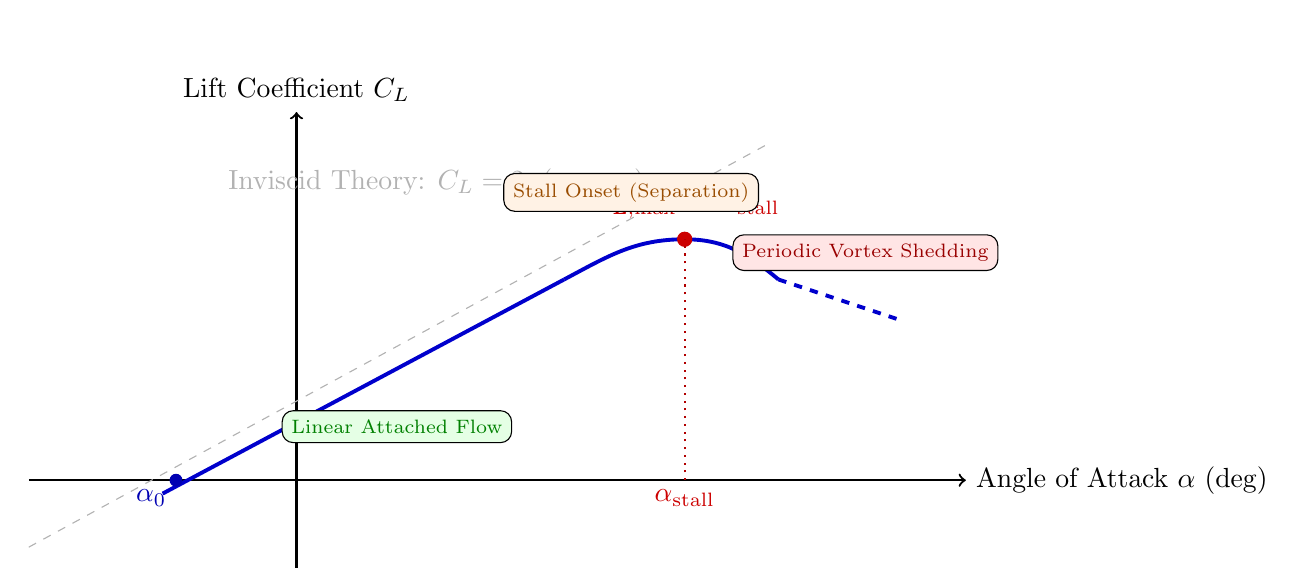
\begin{tikzpicture}[scale=0.85]
    % Axes
    \draw[->, thick] (-4,0) -- (10,0) node[right] {Angle of Attack $\alpha$ (deg)};
    \draw[->, thick] (0,-1.5) -- (0,5.5) node[above] {Lift Coefficient $C_L$};
    
    % Reference lines
    \draw[dashed, gray!60] (-4,-1) -- (7,5.0) node[pos=0.85, above left] {Inviscid Theory: $C_L = 2\pi(\alpha - \alpha_0)$};
    
    % Attached linear region
    \draw[line width=1.4pt, blue!80!black] (-2,-0.2) -- (4,3.0);
    % Curve approaching stall
    \draw[line width=1.4pt, blue!80!black] (4,3.0) to[out=28, in=180] (5.8,3.6) to[out=0, in=140] (7.2,3.0);
    % Deep stall shedding
    \draw[line width=1.4pt, blue!80!black, dashed] (7.2,3.0) -- (9.0,2.4);
    
    % Critical points
    \filldraw[red!80!black] (5.8,3.6) circle (3pt) node[above=4pt] {$\mathbf{C_{L,\max}}$ at $\mathbf{\alpha_{\text{stall}}}$};
    \draw[dotted, red!70!black, thick] (5.8,0) -- (5.8,3.6);
    \node[below, red!80!black] at (5.8,0) {$\alpha_{\text{stall}}$};
    
    % Zero lift angle
    \filldraw[blue!70!black] (-1.8,0) circle (2.5pt) node[below left] {$\alpha_0$};
    
    % Flow regimes annotations
    \node[draw, rounded corners, fill=green!10, text=green!50!black, font=\scriptsize] at (1.5, 0.8) {Linear Attached Flow};
    \node[draw, rounded corners, fill=orange!10, text=orange!60!black, font=\scriptsize] at (5.0, 4.3) {Stall Onset (Separation)};
    \node[draw, rounded corners, fill=red!10, text=red!60!black, font=\scriptsize] at (8.5, 3.4) {Periodic Vortex Shedding};
\end{tikzpicture}
\caption{Anatomy of an aerodynamic lift polar: Linear attached regime, non-linear separation onset, peak lift $C_{L,\max}$ at critical stall angle $\alpha_{\text{stall}}$, and post-stall periodic vortex shedding.}
\label{fig:stall_polar}
\end{figure}

\section{Experimental Testing Platform: NCSSM \textit{WindTunnel lab}}

Tests are conducted using NCSSM's \textbf{WindTunnel lab}, a real-time GPU-accelerated numerical wind tunnel powered by the Lattice Boltzmann Method (LBM D2Q9) and Smagorinsky subgrid-scale turbulence modeling.

\subsection{Standardized Data Acquisition (DAQ) Protocol}
To ensure reproducibility across all student research teams, each data point must be collected according to the \textbf{5-Second Integer Vortex Shedding Integration Protocol}:
\begin{enumerate}
    \item \textbf{Geometry Configuration:} Enter the 4-digit NACA profile (e.g., \texttt{2412}) in the control panel.
    \item \textbf{Flow Conditioning:} Set the target Reynolds number ($Re$) slider and verify that \textit{Smagorinsky LES} is checked.
    \item \textbf{Angle Dialing:} Adjust $\alpha$ using the slider for coarse sweeping ($2.0^\circ$ increments) and the stepper buttons (\texttt{[<]} / \texttt{[>]}) for high-resolution refinement ($0.5^\circ$ increments) in the vicinity of stall.
    \item \textbf{Flow Settling Verification:} Observe the telemetry status indicator. When flow is altered, the indicator displays \textbf{\textcolor{orange}{Flow Settling}}. Wait 3--5 seconds until the badge turns \textbf{\textcolor{green!70!black}{Flow Settled $\cdot$ Ready}}.
    \item \textbf{Execute 5s Cycle Acquisition:} Click \texttt{[Acquire (5s)]} or press hotkey \texttt{L}. The system integrates instantaneous momentum-exchange forces across full shedding periods ($\int \sin(\omega t) dt \equiv 0$), completely filtering phase bias.
    \item \textbf{Telemetry Logging:} The polar graph displays the cycle-averaged $C_L$, accompanied by dynamic error whiskers representing the shedding envelope $[C_{L,\min}, C_{L,\max}]$.
    \item \textbf{CSV Export:} Upon completing an angle sweep, click \texttt{[CSV]} to save the raw laboratory dataset.
\end{enumerate}

\newpage
\section{Consortium Division Assignments}

The class is partitioned into four research divisions. Each division is responsible for executing high-density angle of attack sweeps across their assigned parameter matrix.

\subsection{Division 1: Airfoil Thickness (\texorpdfstring{$t/c$}{t/c}) \& Nose Curvature Division}
\textbf{Primary Objective:} Quantify the impact of leading-edge radius and airfoil thickness on stall onset angle and determine whether thicker profiles experience sudden or docile stall.
\begin{itemize}
    \item \textbf{Fixed Controls:} Baseline Reynolds number $Re = 1000$, Camber $m = 0\%$ (Symmetric Series).
    \item \textbf{Airfoil Sweep Matrix:}
    \begin{enumerate}
        \item \textbf{NACA 0006:} Ultra-thin ($t/c = 6\%$) --- Sharp leading edge, high susceptibility to separation bubble burst.
        \item \textbf{NACA 0009:} Moderately thin ($t/c = 9\%$) --- Classic high-speed profile.
        \item \textbf{NACA 0012:} Standard benchmark ($t/c = 12\%$) --- NASA calibration standard.
        \item \textbf{NACA 0018:} Thick subsonic ($t/c = 18\%$) --- High structural depth, blunt nose.
        \item \textbf{NACA 0024:} Very thick ($t/c = 24\%$) --- Low-speed strut/root section.
    \end{enumerate}
    \item \textbf{Angle Sweep Range:} $\alpha \in [-2.0^\circ,\, +24.0^\circ]$. Sweep in $2.0^\circ$ steps from $-2^\circ$ to $8^\circ$, then $0.5^\circ$ steps from $8^\circ$ to $20^\circ$.
    \item \textbf{Deliverable Plot 1.1:} Composite polar plot ($C_L$ vs $\alpha$) overlaying all five thickness ratios.
    \item \textbf{Deliverable Plot 1.2:} Functional curve of $\alpha_{\text{stall}}$ vs $(t/c)$ and $C_{L,\max}$ vs $(t/c)$.
\end{itemize}

\subsection{Division 2: Airfoil Camber (\texorpdfstring{$m$}{m}) \& Zero-Lift Asymmetry Division}
\textbf{Primary Objective:} Determine how mean camber line curvature shifts the zero-lift angle $\alpha_0$, alters maximum lift $C_{L,\max}$, and affects the stall angle $\alpha_{\text{stall}}$.
\begin{itemize}
    \item \textbf{Fixed Controls:} Baseline Reynolds number $Re = 1000$, Thickness $t/c = 12\%$, Maximum Camber Location $p = 0.4c$ (\texttt{NACA X412} Family).
    \item \textbf{Airfoil Sweep Matrix:}
    \begin{enumerate}
        \item \textbf{NACA 0012:} Symmetric reference ($m = 0\%$).
        \item \textbf{NACA 1412:} Mild camber ($m = 1\%$).
        \item \textbf{NACA 2412:} Benchmark camber ($m = 2\%$, typical general aviation wing).
        \item \textbf{NACA 4412:} High-lift camber ($m = 4\%$).
        \item \textbf{NACA 6412:} Extreme aggressive camber ($m = 6\%$, STOL/cargo section).
    \end{enumerate}
    \item \textbf{Angle Sweep Range:} $\alpha \in [-8.0^\circ,\, +22.0^\circ]$. Sweep in $2.0^\circ$ steps from $-8^\circ$ to $4^\circ$, then $0.5^\circ$ steps through stall.
    \item \textbf{Deliverable Plot 2.1:} Experimental lift slope verification: verify linear slope $dC_L/d\alpha$ against $2\pi$ and plot experimental $\alpha_0$ vs theoretical prediction $\alpha_0 \approx -1.1 m$.
    \item \textbf{Deliverable Plot 2.2:} Functional curve of $\alpha_{\text{stall}}$ vs $m$ and $C_{L,\max}$ vs $m$. Does increasing camber delay or advance stall onset?
\end{itemize}

\subsection{Division 3: Reynolds Number (\texorpdfstring{$Re$}{Re}) \& Viscous Scale Division}
\textbf{Primary Objective:} Determine the empirical scaling law connecting Reynolds number to boundary layer energization and stall angle delay.
\begin{itemize}
    \item \textbf{Fixed Controls:} Standard NACA 2412 airfoil profile ($m=2\%$, $p=0.4c$, $t/c=12\%$).
    \item \textbf{Reynolds Number Sweep Matrix:}
    \begin{enumerate}
        \item \textbf{$Re = 300$:} Viscous-dominated flow (thick laminar boundary layer, micro-aerial scale).
        \item \textbf{$Re = 600$:} Low Reynolds number transitional regime.
        \item \textbf{$Re = 1200$:} Standard baseline tunnel scale.
        \item \textbf{$Re = 2500$:} Moderate Reynolds number with elevated momentum transport.
        \item \textbf{$Re = 5000$:} High Reynolds number testing (energized boundary layer).
    \end{enumerate}
    \item \textbf{Angle Sweep Range:} $\alpha \in [-4.0^\circ,\, +22.0^\circ]$ for each Reynolds number. Focus $0.5^\circ$ resolution in the $[8^\circ, 18^\circ]$ stall zone.
    \item \textbf{Deliverable Plot 3.1:} Family of $C_L(\alpha)$ curves showing the progression of stall softening and delay with increasing $Re$.
    \item \textbf{Deliverable Plot 3.2:} Semilogarithmic scaling plot: $\alpha_{\text{stall}}$ vs $\ln(Re)$ and test for power-law correlation $\alpha_{\text{stall}} \propto Re^k$.
\end{itemize}

\subsection{Division 4: Coupled Interaction \& Post-Stall Shedding Dynamics Division}
\textbf{Primary Objective:} Investigate coupled camber-thickness interactions and quantify dynamic vortex shedding oscillation amplitudes and inverted stall asymmetry.
\begin{itemize}
    \item \textbf{Sweep Matrix A (Coupled Geometry Matrix):}
    \begin{enumerate}
        \item \textbf{NACA 4406:} High camber ($4\%$) + Ultra-thin ($6\%$) --- Severe suction peak combined with sharp nose.
        \item \textbf{NACA 4418:} High camber ($4\%$) + Thick ($18\%$) --- Camber-thickness synergy.
        \item \textbf{NACA 0006 vs NACA 0018:} Thickness extremes under symmetric conditions.
    \end{enumerate}
    \item \textbf{Sweep Matrix B (Bidirectional Inverted Stall Exploration):}
    \begin{enumerate}
        \item Execute a continuous bidirectional sweep on \textbf{NACA 2412} from $\alpha = -16.0^\circ$ to $+20.0^\circ$.
        \item Locate positive stall ($\alpha_{\text{stall}}^+, C_{L,\max}^+$) and inverted negative stall ($\alpha_{\text{stall}}^-, C_{L,\min}^-$).
    \end{enumerate}
    \item \textbf{Deliverable Plot 4.1:} Dynamic shedding envelope diagram: plot oscillation amplitude $\Delta C_L = C_{L,\max} - C_{L,\min}$ (error whiskers) as a function of degrees past stall $(\alpha - \alpha_{\text{stall}})$.
    \item \textbf{Deliverable Plot 4.2:} Cambered airfoil stall asymmetry comparison: contrast positive vs inverted stall modes.
\end{itemize}

\newpage
\section{Classroom Consortium: Multi-Variable Data Pooling}

Following data acquisition, each division will deposit their calibrated data points into the \textbf{Consortium Master Telemetry Database}. Every team will then have access to the complete 4D matrix.

\begin{table}[h!]
\centering
\small
\renewcommand{\arraystretch}{1.2}
\begin{tabular}{@{}llccccc@{}}
\toprule
\textbf{Div.} & \textbf{Airfoil / Case} & $\mathbf{m}$ & $\mathbf{t/c}$ & $\mathbf{Re}$ & \textbf{Meas. } $\mathbf{\alpha_{\text{stall}}}$ (\si{\degree}) & \textbf{Meas. } $\mathbf{C_{L,\max}}$ \\ \midrule
1 & NACA 0006 & 0.00 & 0.06 & 1000 & \rule{1.5cm}{0.15mm} & \rule{1.5cm}{0.15mm} \\
1 & NACA 0009 & 0.00 & 0.09 & 1000 & \rule{1.5cm}{0.15mm} & \rule{1.5cm}{0.15mm} \\
1 & NACA 0012 & 0.00 & 0.12 & 1000 & \rule{1.5cm}{0.15mm} & \rule{1.5cm}{0.15mm} \\
1 & NACA 0018 & 0.00 & 0.18 & 1000 & \rule{1.5cm}{0.15mm} & \rule{1.5cm}{0.15mm} \\
1 & NACA 0024 & 0.00 & 0.24 & 1000 & \rule{1.5cm}{0.15mm} & \rule{1.5cm}{0.15mm} \\ \midrule
2 & NACA 1412 & 0.01 & 0.12 & 1000 & \rule{1.5cm}{0.15mm} & \rule{1.5cm}{0.15mm} \\
2 & NACA 2412 & 0.02 & 0.12 & 1000 & \rule{1.5cm}{0.15mm} & \rule{1.5cm}{0.15mm} \\
2 & NACA 4412 & 0.04 & 0.12 & 1000 & \rule{1.5cm}{0.15mm} & \rule{1.5cm}{0.15mm} \\
2 & NACA 6412 & 0.06 & 0.12 & 1000 & \rule{1.5cm}{0.15mm} & \rule{1.5cm}{0.15mm} \\ \midrule
3 & NACA 2412 ($Re=300$) & 0.02 & 0.12 & 300 & \rule{1.5cm}{0.15mm} & \rule{1.5cm}{0.15mm} \\
3 & NACA 2412 ($Re=600$) & 0.02 & 0.12 & 600 & \rule{1.5cm}{0.15mm} & \rule{1.5cm}{0.15mm} \\
3 & NACA 2412 ($Re=1200$) & 0.02 & 0.12 & 1200 & \rule{1.5cm}{0.15mm} & \rule{1.5cm}{0.15mm} \\
3 & NACA 2412 ($Re=2500$) & 0.02 & 0.12 & 2500 & \rule{1.5cm}{0.15mm} & \rule{1.5cm}{0.15mm} \\
3 & NACA 2412 ($Re=5000$) & 0.02 & 0.12 & 5000 & \rule{1.5cm}{0.15mm} & \rule{1.5cm}{0.15mm} \\ \midrule
4 & NACA 4406 & 0.04 & 0.06 & 1000 & \rule{1.5cm}{0.15mm} & \rule{1.5cm}{0.15mm} \\
4 & NACA 4418 & 0.04 & 0.18 & 1000 & \rule{1.5cm}{0.15mm} & \rule{1.5cm}{0.15mm} \\
4 & NACA 2412 (Inverted) & 0.02 & 0.12 & 1000 & \rule{1.5cm}{0.15mm} & \rule{1.5cm}{0.15mm} \\ \bottomrule
\end{tabular}
\caption{Consortium Master Parametric Telemetry Table for class-wide regression.}
\label{tab:master_table}
\end{table}

\section{Analysis \& Discussion Prompts}

Each research division will author a technical report synthesizing their primary domain and the global consortium dataset. Address the following analytical prompts:

\begin{enumerate}[leftmargin=*]
    \item \textbf{Thickness Scaling \& Optimal Slenderness:}
    Plot $\alpha_{\text{stall}}$ against $(t/c)$ for the symmetric NACA 00XX series.
    \begin{itemize}
        \item At what thickness ratio does $\alpha_{\text{stall}}$ peak?
        \item Physically explain the stall mechanism transition between NACA 0006 (thin-airfoil bubble bursting) and NACA 0018 (progressive trailing-edge stall).
        \item Why does increasing thickness beyond $t/c \approx 0.18$ eventually degrade aerodynamic performance?
    \end{itemize}

    \item \textbf{Camber Effect on Stall vs Lift Capability:}
    Contrast the effect of camber $m$ on $C_{L,\max}$ versus its effect on $\alpha_{\text{stall}}$.
    \begin{itemize}
        \item Does adding camber increase or decrease the stall angle $\alpha_{\text{stall}}$?
        \item Why does NACA 6412 achieve higher $C_{L,\max}$ than NACA 0012 despite intense suction peaks?
        \item Verify Thin Airfoil Theory: calculate the linear regression slope $dC_L/d\alpha$ and compare to $2\pi$. Calculate the zero-lift angle $\alpha_0$ and compare to theoretical $-1.1 m$.
    \end{itemize}

    \item \textbf{Reynolds Scaling and Boundary Layer Energization:}
    Examine the five Reynolds number test points.
    \begin{itemize}
        \item Fit an empirical logarithmic model: $\alpha_{\text{stall}} = A + B \ln(Re/1000)$. Report constants $A$ and $B$ and $R^2$.
        \item Relate your findings to the laminar boundary layer thickness $\delta \propto 1/\sqrt{Re}$. Why does an energized, thinner boundary layer delay separation?
    \end{itemize}

    \item \textbf{Post-Stall Dynamics \& Force Vector Behavior:}
    Observe the real-time vector overlay ($\vec{L}, \vec{D}, \vec{R}$) and smoke streamlines across stall.
    \begin{itemize}
        \item How does the orientation of the resultant force vector $\vec{R}$ rotate as the airfoil transitions into deep stall?
        \item In deep stall, how does the shedding oscillation envelope $[C_{L,\min}, C_{L,\max}]$ relate to the formation and shedding of von K\'{a}rm\'{a}n vortex street structures in the wake?
    \end{itemize}

    \item \textbf{Global Multi-Variable Regression Model:}
    Using the pooled class dataset from Table~\ref{tab:master_table}, fit a multi-linear response surface:
    \begin{equation}
    \alpha_{\text{stall}}\left(m,\, \frac{t}{c},\, Re\right) \approx C_0 + C_m \cdot m + C_t \cdot \left(\frac{t}{c}\right) + C_{Re} \cdot \ln\left(\frac{Re}{1000}\right).
    \end{equation}
    Determine the regression coefficients $C_0, C_m, C_t, C_{Re}$ and discuss the dominant sensitivity governing stall onset in subsonic flight.
\end{enumerate}

\section{Grading Rubric (100 Points Total)}

\begin{table}[h!]
\centering
\small
\renewcommand{\arraystretch}{1.2}
\begin{tabular}{@{}p{3.8cm}p{9.4cm}c@{}}
\toprule
\textbf{Criterion} & \textbf{Performance Expectations} & \textbf{Points} \\ \midrule
\textbf{Experimental Protocol \& DAQ Rigor} & Correct execution of 5s burst integration protocol; flow settled state verified; appropriate angle density ($0.5^\circ$ near stall); complete CSV exports. & 20 \\
\textbf{Data Visualization \& Polar Curves} & Clear, publication-grade polar plots ($C_L$ vs $\alpha$, $C_D$ vs $\alpha$, $L/D$ vs $\alpha$) with error whiskers, stall points clearly identified, theoretical references included. & 20 \\
\textbf{Physical Mechanisms \& Fluid Dynamics} & Sound, thorough physical reasoning explaining separation, suction peaks, boundary layer energy, vortex shedding, and thin vs trailing-edge stall. & 25 \\
\textbf{Consortium Synthesis \& Regression} & Successful integration with class dataset; formulation and statistical evaluation of the multi-variable scaling model $\alpha_{\text{stall}} = \Phi(m, t/c, Re)$. & 20 \\
\textbf{Technical Communication \& Formatting} & Clear engineering report organization; proper unit annotations; professional tables, diagrams, and executive summary. & 15 \\ \midrule
\textbf{Total} & & \textbf{100} \\ \bottomrule
\end{tabular}
\caption{Laboratory Evaluation and Assessment Rubric.}
\label{tab:rubric}
\end{table}

\end{document}
